%!TEX root = main.tex
We demonstrate the performance and capability of Bempp-Exafmm via electrostatic simulations, including computing the solvation energy of a Zika virus.
This section presents five types of results.
The first result explains the behavior of two variants of the mathematical formulation, from the conditioning point of view. 
Second, we show solution verification through two grid-convergence studies: with a spherical molecule (having an analytical solution), and with a real biomolecule (using Richardson extrapolation).
Third, we compare our results with those obtained from the APBS package using 8 other molecules.
The fourth type of result looks at performance with problem sizes between 8,000 and 2 million elements, including timings, breakdowns, and computational complexity.
Our final result is a demonstration using a structure with about 1.6 million atoms, the Zika virus, discretized with about 10 million boundary elements.

We ran all experiments on a single CPU node of \textit{Pegasus}, a Linux cluster at the George Washington University.
Each node is equipped with two 20-core Intel Xeon Gold 6148 CPUs (base frequency at 2.4 GHz, max turbo frequency at 3.7 GHz) and 192GB RAM.
All runs are based on Bempp-cl version 0.2.2 and Exafmm-t version 0.1.0.
We compiled Exafmm with Intel compiler (version 19.0.5.281) and enabled \texttt{-xHost} option for vectorization.
We used the full GMRES from the SciPy library as our linear solver.

In all of the following test cases, the relative permittivity is $\epsilon_1 = 4$ in the solute region and $\epsilon_2 = 80$ in the solvent region, and the inverse of Debye length in the solvent region is $\kappa = 1/8\ {\si{\angstrom}}^{-1}$.
We downloaded the molecule structures from the Protein Data Bank (PDB), parameterized them with \texttt{pdb2pqr}~\cite{DolinskyETal2004}, and generated meshes on the solvent-excluded surface (SES) using \texttt{Nanoshaper} with a probe radius of $1.4 \si{\angstrom}$.

\paragraph{Matrix conditioning of two derivative formulations} \label{result_conditioning}
Section \ref{s:formulation} presents the two formulations to solve the integral equations  \eqref{eq:volume_potential} derived from the Poisson-Boltzmann model of biomolecular electrostatics: 
the \emph{direct}~\cite{YoonLenhoff1990}  and \emph{derivative}~\cite{JufferETal1991} formulations.
The latter is well-known to lead to a better-conditioned matrix.
Its most common solution method finds the potential and its derivative in the interior of the boundary via equations \eqref{eq:juffer}, but an alternative is to solve for the exterior fields via \eqref{eq:lu}.
Bempp unfetters the user to experiment with these variants of the boundary element solution method, editing just a few lines of Python.
We could easily try both the interior and exterior versions of the derivative formulation, whereas previous publications opted for one method and used it throughout.
The programming effort required to implement a second formulation would have been a good reason.
In our experiments, the exterior version used by Lu and coworkers~\cite{LuETal2006,LuETal2009,ZhangETal2019} took about half as many iterations to converge than the interior version---a sizable advantage.
This led us to study the properties of the two variants of the derivative formulation in more detail.
The results in this section aim to give a simple explanation for the different numerical behavior of the two methods.
Our ability to explore and explain this issue showcases the power of interactive computing with a high-productivity software platform, like that provided by Bempp-Exafmm.

GMRES methods have an intricate convergence behavior \cite{mark1999a}.
Heuristically, if the eigenvalues are clustered with the cluster being sufficiently far away from the origin, we expect fast convergence of GMRES to the desired solution.
Figures \ref{fig:derivative_interior_eig} and \ref{fig:derivative_exterior_eig} show the eigenvalues of the interior and exterior derivative formulations, respectively, on the complex plane.
With the interior formulation, eigenvalues cluster around two points, while eigenvalues cluster around only one point with the exterior formulation.

The difference is due to the diagonal of the corresponding system of integral equations.
In the case of the interior formulation, the associated left-hand side operator takes the form
$$
\begin{bmatrix}\frac{1}{2}(1 + \frac{\epsilon_2}{\epsilon_1})I & 0 \\ 0 & \frac{1}{2}(1 + \frac{\epsilon_1}{\epsilon_2})I
\end{bmatrix} + \mathcal{C}_{int},
$$
where $\mathcal{C}_{int}$ is a compact operator on sufficiently smooth domains. (On smooth domains the single-layer, double-layer and adjoint double-layer operators are compact operators.
Furthermore, the difference of the hypersingular operators is compact \cite{Hiptmair2006-om}.)
The eigenvalues of the interior derivative operator hence accumulate at the points $\frac{1}{2}(1 + \frac{\epsilon_2}{\epsilon_1})$ and $\frac{1}{2}(1 + \frac{\epsilon_1}{\epsilon_2})$.
In contrast, the exterior derivative operator has the form
$$
\begin{bmatrix}\frac{1}{2}(1 + \frac{\epsilon_1}{\epsilon_2})I & 0 \\ 0 & \frac{1}{2}(1 + \frac{\epsilon_1}{\epsilon_2})I
\end{bmatrix} + \mathcal{C}_{ext},
$$
where $\mathcal{C}_{ext}$ is again a compact operator.
We now only have one accumulation point, namely $\frac{1}{2}(1 + \frac{\epsilon_1}{\epsilon_2})$.
Unless $\epsilon_1\approx \epsilon_2$ we therefore expect the eigenvalues to be much closer together than in the interior derivative case and therefore the GMRES convergence to be faster for the exterior derivative formulation.

We want to emphasize that the above argument is valid for the continuous operators.
Under discretization, the resulting eigenvalue problem is of the form $A\mathbf{x}=\lambda M\mathbf{x}$ (or equivalently $M^{-1}A\mathbf{x}=\lambda \mathbf{x}$, where $A$ is the $2\times 2$ block operator associated with the Galerkin discretization of the integral operator system and $M = \text{diag}(\hat{M}, \hat{M})$ is a block diagonal mass matrix, where the matrix $\hat{M}$ is the matrix containing the surface inner products $\int_{\Gamma}\psi_i(\mathbf{r})\phi_j(\mathbf{r})ds(\mathbf{r})$ for test functions $\psi_j$ and trial functions $\phi_i$ (which are both chosen as continuous, piecewise linear basis functions for the derivative formulation in this paper).
The mass-matrix preconditioned linear system of equations to solve has the form $M^{-1}A\mathbf{x} = M^{-1}\mathbf{b}$ for vector of unknowns $\mathbf{x}$ and right-hand side $\mathbf{b}$ and Figures \ref{fig:derivative_interior_eig} and \ref{fig:derivative_exterior_eig} show the eigenvalues of $M^{-1}A$ for the interior and exterior derivative formulation.
In practice, the action of $M^{-1}$ can be computed through a sparse LU decomposition of $M$.
However, for problems with millions of unknowns this is becoming expensive.
For practical electrostatic computations we have therefore chosen a simple mass lumping approach, in which we substitute $M$ by a diagonal matrix, where each diagonal entry is the sum of the corresponding row values of $M$.
This diagonal matrix can then be trivially inverted.
In our experiments the mass lumping only led to a modest increase in the number of iterations compared to using the LU decomposition of the mass matrix $M$.
We stress that mass matrix preconditioning is necessary to solve the interior and exterior formulations in a reasonable number of iterations.
The approximation of the inverse of the mass matrix $M$ through mass lumping only affects the preconditioner and not the solution of the underlying linear system of equations itself.

In each of the following studies, we present two sets of results: one from using the exterior derivative formulation with piecewise linear elements, preconditioned by a mass lumping matrix, and the other from using the direct formulation with piecewise constant elements, preconditioned by a block-diagonal matrix presented by Altman and co-workers \cite{AltmanBardhanWhiteTidor2009}.


\begin{figure*}
    \begin{center}
        \subfloat[][]{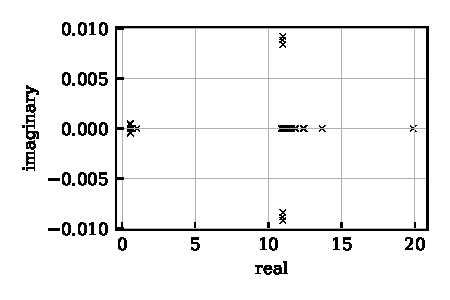
\includegraphics[width=0.4 \textwidth]{derivative_interior_eig.pdf}
        \label{fig:derivative_interior_eig}}\qquad
        \subfloat{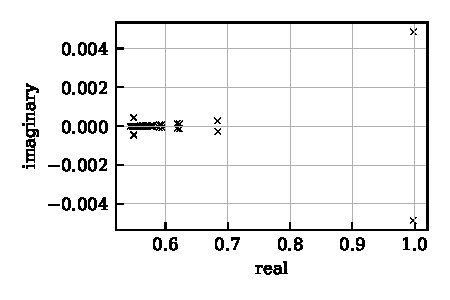
\includegraphics[width=0.4 \textwidth]{derivative_exterior_eig.pdf}
        \label{fig:derivative_exterior_eig}}
    \end{center}
    \caption{Eigenvalues of the system matrix of the derivative formulation for interior field (\textbf{a}) and for exterior field (\textbf{b}).
    }
\end{figure*}

\paragraph{Mesh refinement study using a spherical molecule} \label{result_convergence_sphere}

As a form of solution verification with the Bempp-Exafmm software, we completed two mesh-refinement studies.
The first used a spherical molecule with an off-center charge, for which we have an analytical solution.
In the next sub-section, we present a mesh-refinement study with a real molecule of biological relevance.
Figure \ref{fig:sketch_sphere_convergence} depicts the problem setup for the current case:
a spherical molecule of radius 4 \AA\ and relative permittivity $\epsilon_1 = 4$, with a unit charge located at $(1,1,1)$.
The solvent region has the relative permittivity of water ($\epsilon_2 = 80$), and a salt concentration of $150$mM $(\kappa = 1/8\ {\si{\angstrom}}^{-1})$.
Other simulation parameters are listed in Table \ref{tab:convergence}.
With an expansion order of 10, our \fmm achieved 9 digits of accuracy.
We computed the solvation energy of this molecule using $5$ different meshes, obtained using a constant refinement factor of 4.

\begin{table}[]
    \centering
    \begin{tabular}{lc}
    \hline
    \gmres tolerance          & $10^{-7}$ \\
    \# regular quadrature points  & 6    \\
    \fmm expansion order      & 10   \\
    \fmm $\ncrit$             & 500  \\
    \hline  \vspace{0.3 cm}
    \end{tabular}

    \begin{tabular}{cc}
    number of elements & mesh density ($\#/{\si{\angstrom}}^2$) \\
    \hline
    3032               & 1                                       \\
    6196               & 2                                       \\
    12512              & 4                                       \\
    25204              & 8                                       \\
    50596              & 16                                     
    \end{tabular}
    \caption{Simulation parameters for the grid-refinement studies (top); mesh sizes/densities used in the grid refinement study on 5PTI. Mesh densities measured as number of elements per square Angstrom.}
    \label{tab:convergence}
\end{table}

Kirkwood's derivation \cite{kirkwood1934theory} allows us to compute the analytical solution for the solvation energy in this case, to compare with the numerical result: $-12.258363$ [kcal/mol].
Figure \ref{fig:sphere_convergence} shows the error in the solvation energy, converging at the expected rate of $1/N$ for both formulations.
The observed order of convergence is 1.001 for the direct formulation and 0.999 for the derivative formulation, using the middle three values.

\paragraph{Mesh refinement study using 5PTI} \label{result_convergence_5PTI}

Next, we tested our software using a real biomolecule: bovine pancreatic trypsin inhibitor (PDB code 5PTI), whose structure \cite{wlodawer1984structure} is shown in Figure \ref{fig:5PTI_structure}.
We parameterized the molecule with \texttt{pdb2pqr} and the \texttt{charmm} force field, and then computed the solvation energy using 5 meshes with the element density ranging from 1 to 16 (Table \ref{tab:convergence}).
This test used the same parameters listed in Table \ref{tab:convergence}, which are fine enough to reveal the discretization error.
Since an analytical solution is not available for this geometry, we obtained the reference values for error estimation via Richardson extrapolation.
The estimated relative error with the finest mesh is 1.2\% with the direct formulation, and 1.5\% with the derivative formulation.



Figure \ref{fig:5PTI_convergence} shows that the error of the computed solvation energy for 5PTI converges linearly with respect to $N$.
The observed order of convergence is 1.156 for the direct formulation and 1.038 for the derivative formulation, using the middle three values.
Both convergence results provide solution verification, and are evidence that our software solves the mathematical model correctly.

\begin{figure*}
        \centering
     \subfloat[][Sphere with an off-center unit charge at $(1,1,1)$.]{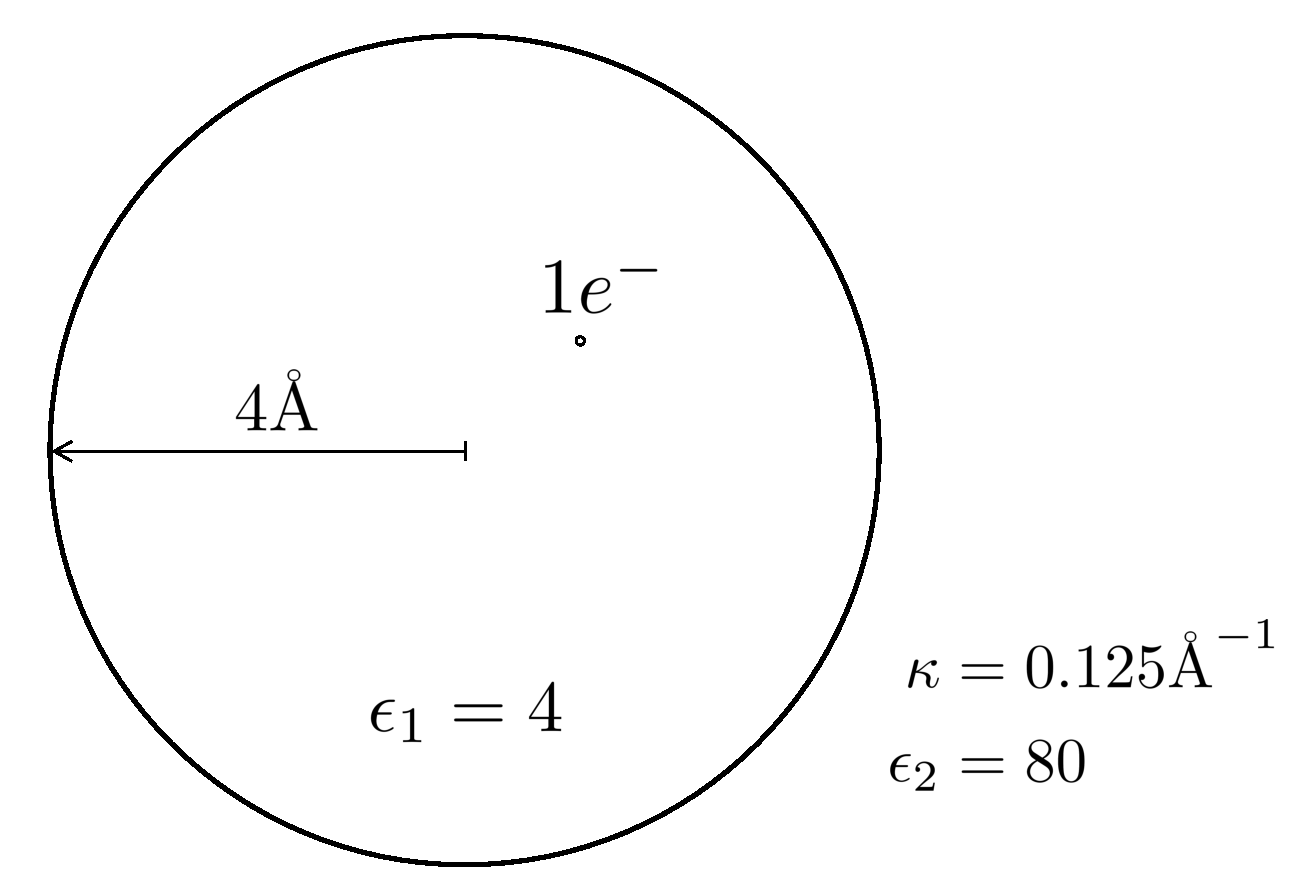
\includegraphics[width=0.4 \textwidth]{sketch_sphere_convergence.pdf}
        \label{fig:sketch_sphere_convergence}}\quad
     \subfloat[][Structure of 5PTI.]{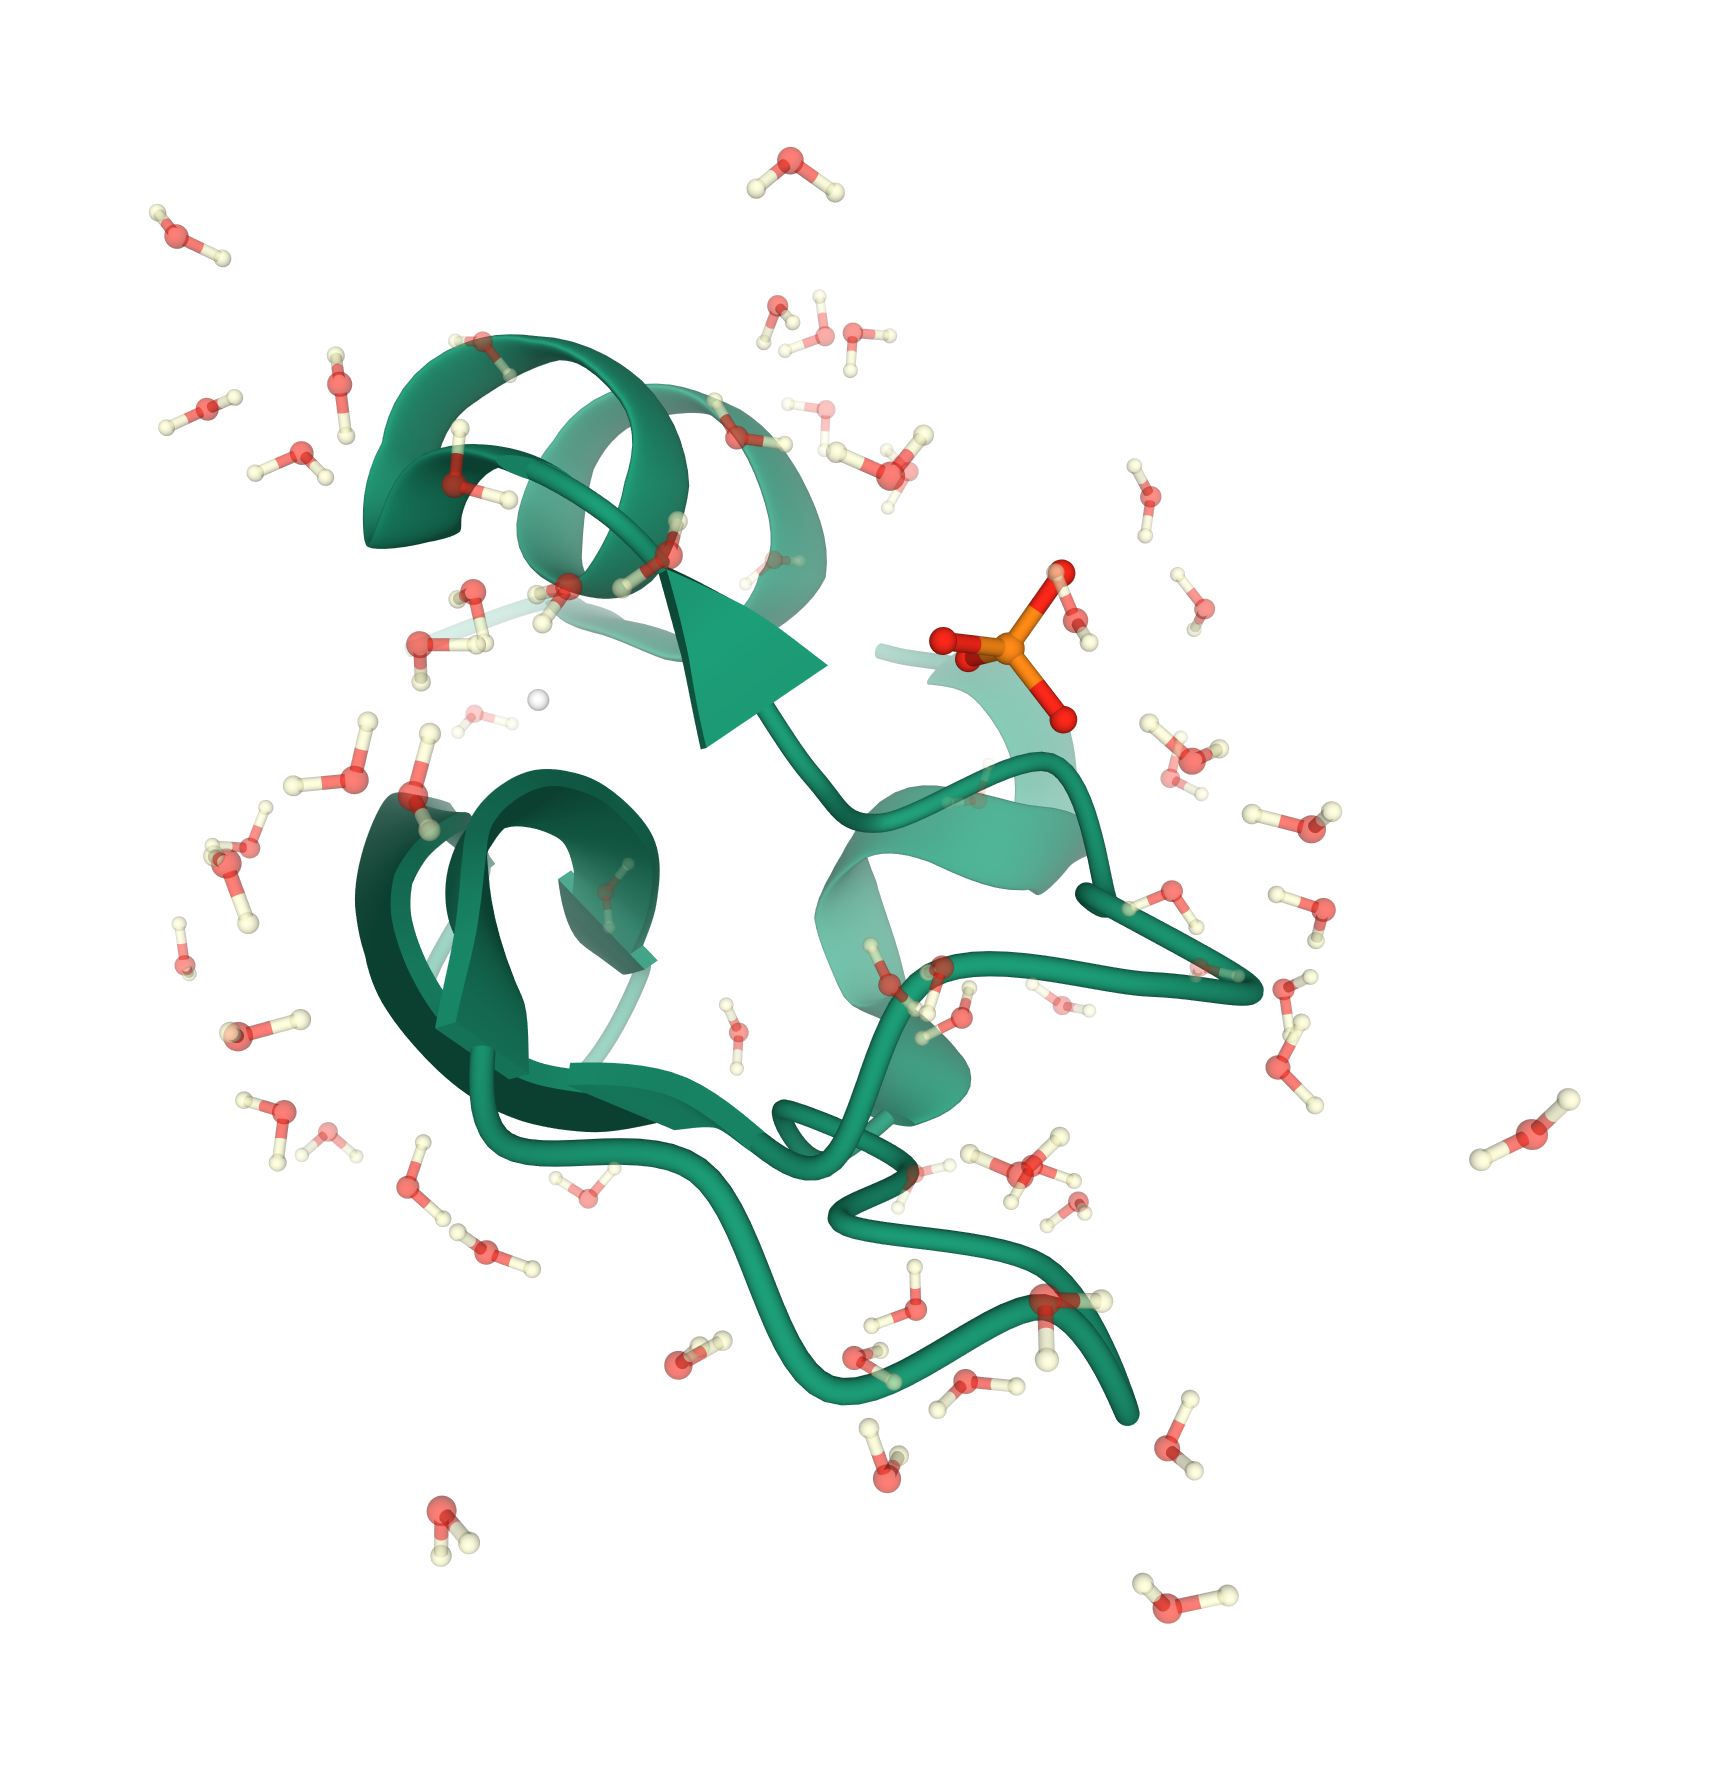
\includegraphics[width=0.35 \textwidth]{5PTI.png}
        \label{fig:5PTI_structure}}\\
     \subfloat[][]{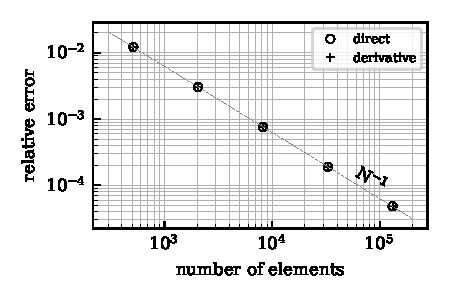
\includegraphics[width=0.4 \textwidth]{sphere_convergence.pdf}
        \label{fig:sphere_convergence}}
     \subfloat[][]{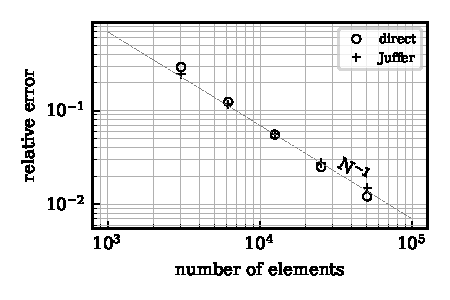
\includegraphics[width=0.4 \textwidth]{5PTI_convergence.pdf}
        \label{fig:5PTI_convergence}}
    \caption{Mesh refinement studies using a spherical molecule and a real biomolecule: bovine pancreatic trypsin inhibitor (PDB code 5PTI).
    \textbf{c}, Mesh convergence study on a spherical molecule with an off-center charge, using both direct formulation and derivative formulation. The error on the solvation energy with respect to the analytical solution is plotted for five meshes:
    the sphere discretized with 512, 2048, 8192, 32768 and 131072 boundary elements.
    \textbf{d}, Mesh convergence study of the solvation energy of bovine pancreatic trypsin inhibitor (PDB code 5PTI), using both direct formulation and derivative formulation.
    The error is with respect to the extrapolated solution using Richardson extrapolation.
    }
\end{figure*}

% add comparison with results from APBS
\paragraph{Comparison with trusted community software} \label{comparison}
We build more confidence on Bempp-Exafmm by comparing our results with a well-established finite-difference code APBS (version 1.5), using 5PTI and 8 other molecules.
We prepared the molecular structures using the \texttt{charmm} force field.
For each molecule, we created three successive meshes for each software to study the convergence.
For Bempp-Exafmm, we used \texttt{Nanoshaper} to generate three surface meshes with the element density set to 4, 8, 16 ${\si{\angstrom}}^{-2}$, respectively.
In APBS, we controlled the multigrid parameters to ensure that three grid spacings are refined with a constant factor of 2.
All mesh sizes are listed in Appendix \ref{sec:apbs_mesh}.
Other parameters are the same as our previous grid-convergence study, as listed in Table \ref{tab:convergence}.

Table \ref{tab:APBS_result} presents the convergence results of both codes using a set of molecules.
The derivative formulation is used in Bempp.
We obtained an extrapolated value of the solvation energy of each molecule, serving as the reference value, for each software, respectively.
As expected, the solvation energy computed from Bempp converges at the rate of $\mathcal{O}(N^{-1})$, where $N$ is the number of elements.
With APBS, the average observed order of convergence over all cases is 1.25, with respect to the grid spacing $h$, and other studies \cite{CooperBardhanBarba2014,GengKrasny2013} have reported a similar rate. 
Our $\mathcal{O}(N^{-1})$ convergence corresponds to $\mathcal{O}(h^{-2})$ convergence in element size.
The difference of the extrapolated solvation energy between two codes varies between 0.8\% and 1.8\% across all cases.
This discrepancy is expected because Bempp-Exafmm and APBS use different geometrical representations for the molecular surface, and furthermore, the atomic charges in the molecule are mapped to grid points through interpolation in APBS.
We also compared our results with MIBPB \cite{chen2011mibpb} only using the finest mesh, and the details can be found in Appendix \ref{sec:comp_mibpb}.

\begin{table*}[]
    \centering
    \resizebox{\textwidth}{!}{%
    \begin{tabular}{cc|ccc|cc|ccc|cc}
      &   & \multicolumn{5}{c|}{APBS}                                                                    & \multicolumn{5}{c}{Bempp}                                                                   \\
      &   & \multicolumn{3}{c|}{Error}     & \multirow{2}{*}{$\Delta G_{solv}$} & \multirow{2}{*}{Order$(1/h)$} & \multicolumn{3}{c|}{Error}     & \multirow{2}{*}{$\Delta G_{solv}$} & \multirow{2}{*}{Order$(1/N)$} \\
    ID   & $N_{atoms}$ & coarse   & medium   & fine     &                                    &                        & coarse   & medium   & fine     &                                    &                        \\ \hline
    1AJJ & 513 & 4.40e-02 & 1.33e-02 & 4.00e-03 & -266.15                            & 1.73                   & 2.75e-02 & 1.12e-02 & 4.59e-03 & -268.67                            & 1.29                   \\
    1VJW & 826 & 3.09e-02 & 1.45e-02 & 6.77e-03 & -297.06                            & 1.09                   & 4.92e-02 & 2.23e-02 & 1.01e-02 & -302.50                            & 1.14                   \\
    5PTI & 892 & 3.68e-02 & 1.38e-02 & 5.14e-03 & -311.69                            & 1.42                   & 5.12e-02 & 2.23e-02 & 9.67e-03 & -314.34                            & 1.20                   \\
    1R69 & 997 & 4.31e-02 & 2.10e-02 & 1.02e-02 & -261.02                            & 1.04                   & 5.09e-02 & 2.34e-02 & 1.08e-02 & -265.02                            & 1.12                   \\
    1A2S & 1272 & 5.25e-02 & 2.40e-02 & 1.10e-02 & -456.56                            & 1.13                   & 4.21e-02 & 1.93e-02 & 8.86e-03 & -461.25                            & 1.12                   \\
    1SVR & 1433 & 5.28e-02 & 2.21e-02 & 9.28e-03 & -393.45                            & 1.25                   & 6.48e-02 & 2.89e-02 & 1.29e-02 & -398.83                            & 1.16                   \\
    1A63 & 2065 & 4.51e-02 & 1.88e-02 & 7.82e-03 & -559.39                            & 1.26                   & 5.82e-02 & 2.60e-02 & 1.16e-02 & -567.24                            & 1.16                   \\
    1A7M & 2804 & 4.13e-02 & 1.88e-02 & 8.53e-03 & -524.29                            & 1.14                   & 4.93e-02 & 2.24e-02 & 1.02e-02 & -531.48                            & 1.14                   \\
    1F6W & 8247 & 6.45e-02 & 2.78e-02 & 1.20e-02 & -1277.51                           & 1.21                   & 4.18e-02 & 1.80e-02 & 7.76e-03 & -1301.08                           & 1.22                     
    \end{tabular}
    }
    \caption{Convergence results of the solvation energy of 9 molecules using APBS and Bempp with derivative formulation.
    The error is with respect to an extrapolated value of the solvation energy using Richardson extrapolation.
    The solvation energy $\Delta G_{solv}$ is in units of kcal/mol.
    The observed order of convergence is with respect to the grid spacing $h$ for APBS (volumetric-based) and with respect to the number of elements $N$ for Bempp (boundary-element-based).}
    \label{tab:APBS_result}
\end{table*}


\paragraph{Performance study with direct and derivative formulations} \label{result_performance}

In this sub-section, we investigate the computational performance of Bempp-Exafmm using a spherical molecule.
The sphere has a radius of 1 \AA\, and 100 charges are placed randomly inside, representing the atoms in the solute.
We used the same dielectric constants and salt concentration as in previous grid-convergence studies.
Other simulation parameters are listed in Table \ref{tab:sim_params_performance}.

\begin{table}[]
    \centering
    \begin{tabular}{lc}
    \hline
    \gmres tolerance          & $10^{-4}$ \\
    \# regular quadrature points  & 6    \\
    \fmm expansion order      & 5   \\
    \fmm $\ncrit$             & 500  \\
    \hline
    \end{tabular}
    \caption{Simulation parameters used in the performance study for a spherical molecule.}
    \label{tab:sim_params_performance}
\end{table}

To cover a wide range of problem sizes, we used five surface discretizations, with the number of elements ranging from 8 thousand to 2 million.
Table \ref{tab:sphere_time} presents the assembly time, the solution time and the number of iterations to converge in each case for both formulations.
The assembly time includes the time to pre-compute the \fmm invariant matrices, create sparse and singular assemblers and calculate preconditioners.
The algebraic convergence shows that the condition number grows as the problem size increases with the direct formulation, while it remains at the same level with the derivative formulation.

\begin{table*}[]
    \centering
    \begin{tabular}{c|cccc|cccc}
                                                                 & \multicolumn{4}{c|}{direct}                                                                                                                                                                       & \multicolumn{4}{c}{derivative}                                                                                                                                                                        \\ \hline
    \begin{tabular}[c]{@{}c@{}}number of\\ elements\end{tabular} & \begin{tabular}[c]{@{}c@{}}total\\ time (s)\end{tabular} & \begin{tabular}[c]{@{}c@{}}assembly\\ time (s)\end{tabular} & \begin{tabular}[c]{@{}c@{}}GMRES\\ time (s)\end{tabular} & \# iterations & \begin{tabular}[c]{@{}c@{}}total\\ time (s)\end{tabular} & \begin{tabular}[c]{@{}c@{}}assembly\\ time (s)\end{tabular} & \begin{tabular}[c]{@{}c@{}}GMRES\\ time (s)\end{tabular} & \# iterations \\ \hline
    8192                                                         & 14.0                                                     & 5.4                                                         & 8.6                                                      & 20            & 16.1                                                     & 9.6                                                         & 6.5                                                      & 5            \\
    32768                                                        & 35.1                                                     & 11.7                                                        & 23.4                                                     & 24            & 35.5                                                     & 22.2                                                        & 13.3                                                     & 4            \\
    131072                                                       & 144.2                                                    & 32.8                                                        & 111.4                                                    & 34            & 114.7                                                    & 67.2                                                        & 47.5                                                     & 4            \\
    524288                                                       & 675.8                                                    & 121.6                                                       & 554.2                                                    & 51            & 421.3                                                    & 256.3                                                       & 165.0                                                    & 4            \\
    2097152                                                      & 3159.8                                                   & 483.3                                                       & 2676.5                                                   & 70            & 1592.1                                                   & 1011.6                                                      & 580.5                                                    & 4           
    \end{tabular}
    \caption{Assembly and solution times of calculating the solvation energy of a spherical molecule with 100 random charges inside, using the direct and derivative (exterior) formulations.
    6 regular quadrature points were used per element and the \fmm expansion order was set to 5.}
    \label{tab:sphere_time}
\end{table*}

In our implementation, each iteration in direct formulation requires $8$ \fmm evaluations, whereas each iteration in the derivative formulation requires 19, making it more than twice as expensive.
That explains why the direct formulation leads to a shorter solution time (\gmres time), despite a slower convergence, in the two smaller cases.
For larger problem sizes, faster convergence in the derivative formulation offsets the larger cost per iteration.

As for the assembly time, the derivative formulation is about $2\times$ slower, since it needs to construct twice as many operators as the direct formulation.
In addition, the two hypersingular operators make it even more involved.
Figure \ref{fig:sphere_assembly_time} shows the linear scaling of the assembly time with respect to $N$.

Next, we want to confirm that the time complexity of mat-vecs in \gmres is also $\mathcal{O}(N)$.
The Poisson equation requires \fmm with Laplace kernel and the linearized Poisson-Boltzmann equation requires \fmm with Yukawa kernel.
As we mentioned before, each iteration involves multiple \fmm evaluations: 4 Laplace {\fmm}s and 4 Yukawa {\fmm}s for the direct formulation, 8 and 11 for the derivative formulation.
We averaged the time spent on 1 Laplace \fmm and 1 Yukawa \fmm respectively using direct formulation, and plotted it with respect to $N$ in Figure \ref{fig:sphere_fmm}.
Using an \fmm order of 5, we achieved about 5 digits of accuracy in each mat-vec.
The timings and linear scaling substantiate the efficiency of our \fmm implementation.
In the largest case with over 12 million quadrature points, one Laplace \fmm costs $2.1$s and one Yukawa \fmm costs $5.4$s to compute.

In Bempp, the matrix-vector product has the shape $A\mathbf{x} = P_2^T (G - C)P_1 \mathbf{x} + S \mathbf{x}$ (see Equation \ref{eq:bempp_fmm_matvec}), where the dominant costs are the \fmm evaluation of the Green's function matrix $G$ and the on-the-fly evaluation of the singular correction matrix $C$. Moreover, as stated above for the full $2\times 2$ block system a number of \fmm passes together with corresponding singular corrections need to be performed.
Therefore, the \gmres time reported here consists of \fmm time, singular correction time, as well as the time spent on other steps in the \gmres algorithm.
Figure \ref{fig:sphere_gmres_direct} and \ref{fig:sphere_gmres_derivative} show the time breakdown of \gmres in percentages.
As problem size increases, \fmm evaluations dominate the solution time.

We also measured the peak memory usage using the GNU time command \texttt{/usr/bin/time -v}. (Some Linux distributions do not ship with GNU time.)
We observed a linear space complexity as shown in Figure \ref{fig:sphere_memory}.
The largest case, with more than $2$ million elements, requires $36$GB for the direct formulation and $43$GB for the derivative formulation.

\begin{figure*}[t]
\centering
    \subfloat[][Assembly time]{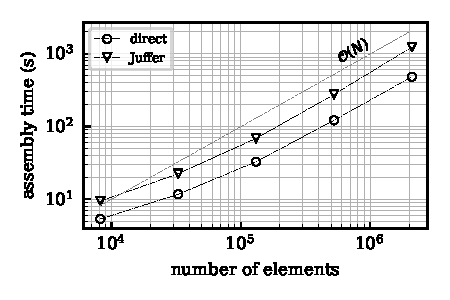
\includegraphics[width=0.33\textwidth]{sphere_assembly_time.pdf}
        \label{fig:sphere_assembly_time}}
   \subfloat[][Average evaluation time.]{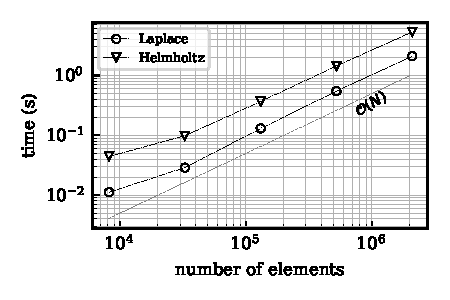
\includegraphics[width=0.33\textwidth]{sphere_fmm.pdf}
        \label{fig:sphere_fmm}}
    \subfloat[][Overall memory consumption in GB.]{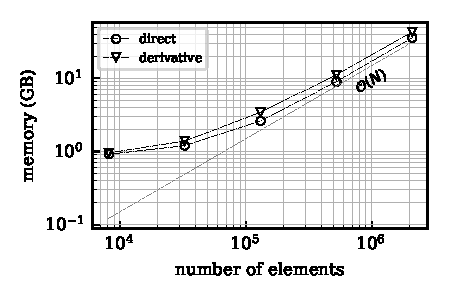
\includegraphics[width=0.33\textwidth]{sphere_memory.pdf}
        \label{fig:sphere_memory}}\\
    \subfloat[][]{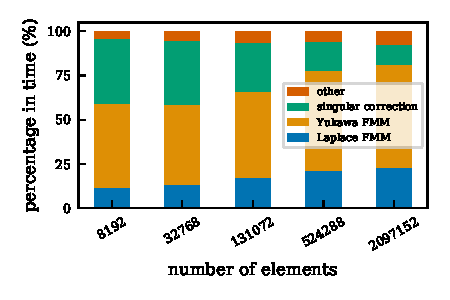
\includegraphics[width=0.4\textwidth]{sphere_gmres_direct.pdf}
        \label{fig:sphere_gmres_direct}}
  \subfloat[][]{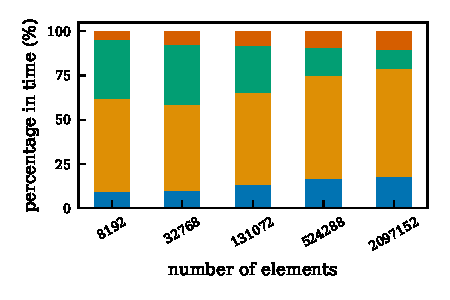
\includegraphics[width=0.4\textwidth]{sphere_gmres_derivative.pdf}
        \label{fig:sphere_gmres_derivative}}
    \caption{Performance on a spherical molecule with 100 random charges inside;
    6 regular quadrature points per element; \fmm expansion order set to 5 to achieve 5 digits of accuracy. Problem size represented by number of elements, $N$. Evaluation time (b) is an average for 1 Laplace \fmm evaluation and 1 Yukawa \fmm evaluation across all iterations in GMRES using direct formulation.
    \textbf{c},\textbf{d}, Time breakdown of \gmres in percentage using direct formulation (\textbf{c}) and derivative formulation (\textbf{d}).}
\end{figure*}

\paragraph{Solvation energy of a Zika virus} \label{result_zika}

Finally, we present a more challenging problem that studies the solvation energy of the Zika virus (PDB code 6CO8), whose structure \cite{sevvana2018refinement} is shown in Figure \ref{fig:6CO8_assembly}.
We parameterized the molecular structure with the \texttt{amber} force field, and generated a mesh on the SES using \texttt{Nanoshaper}. (Mesh generation took less than 5 min.)
The prepared structure contains about 1.6 million atoms and our mesh has around 10 million boundary elements and a total surface area of $3.14\times 10^6 {\si{\angstrom}}^{2}$, corresponding to an element density of $3.16 {\si{\angstrom}}^{-2}$.
In this experiment, 3 quadrature points were used for regular Galerkin integrals over disjoint elements.
The \fmm expansion order was set to 4 obtain 4 digits of accuracy in mat-vecs and the tolerance of \gmres was $10^{-4}$.

\begin{table*}[]
    \centering
    \begin{tabular}{c|c|ccccc}
                 & \begin{tabular}[c]{@{}c@{}}$\Delta G_{\mathrm{solv}}$\\ (kcal/mol)\end{tabular} & \begin{tabular}[c]{@{}c@{}}total \\ time (s)\end{tabular} & \begin{tabular}[c]{@{}c@{}}assembly \\ time (s)\end{tabular} & \begin{tabular}[c]{@{}c@{}}GMRES \\ time (s)\end{tabular} & \begin{tabular}[c]{@{}l@{}}memory\\ (GB)\end{tabular} & \# iterations \\ \hline
    direct     & -116587.5                                               & 11005.4                                                   & 1534.5                                                       & 9470.9                                                    & 109.7                                                 & 105           \\
    derivative & -116254.9                                               & 8370.3                                                    & 3553.9                                                       & 4816.4                                                    & 152.0                                                 & 18            
    \end{tabular}
    \caption{Results of computing the solvation energy of a Zika virus with Bempp using both the direct and derivative formulations.
    3 regular quadrature points were used per element and the \fmm expansion order was set to 4.
    The mesh generation time is minor and not included in the total time.
    To verify our result, we ran the same case with \pygbe using the direct formulation on a workstation with a 24-core CPU.
    The solvation energy computed from \pygbe is -117261.1 [kcal/mol].
    }
    \label{tab:6CO8_result}
\end{table*}

\begin{figure*}
    \subfloat[][]{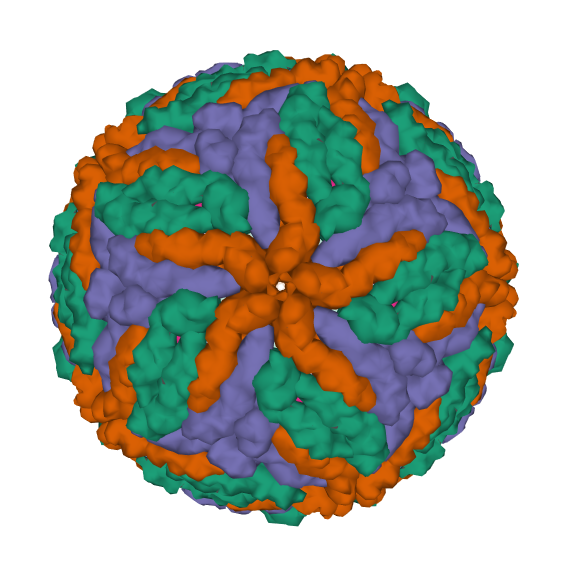
\includegraphics[width=0.25\textwidth]{6CO8_assembly.png}
        \label{fig:6CO8_assembly}}
\subfloat[][]{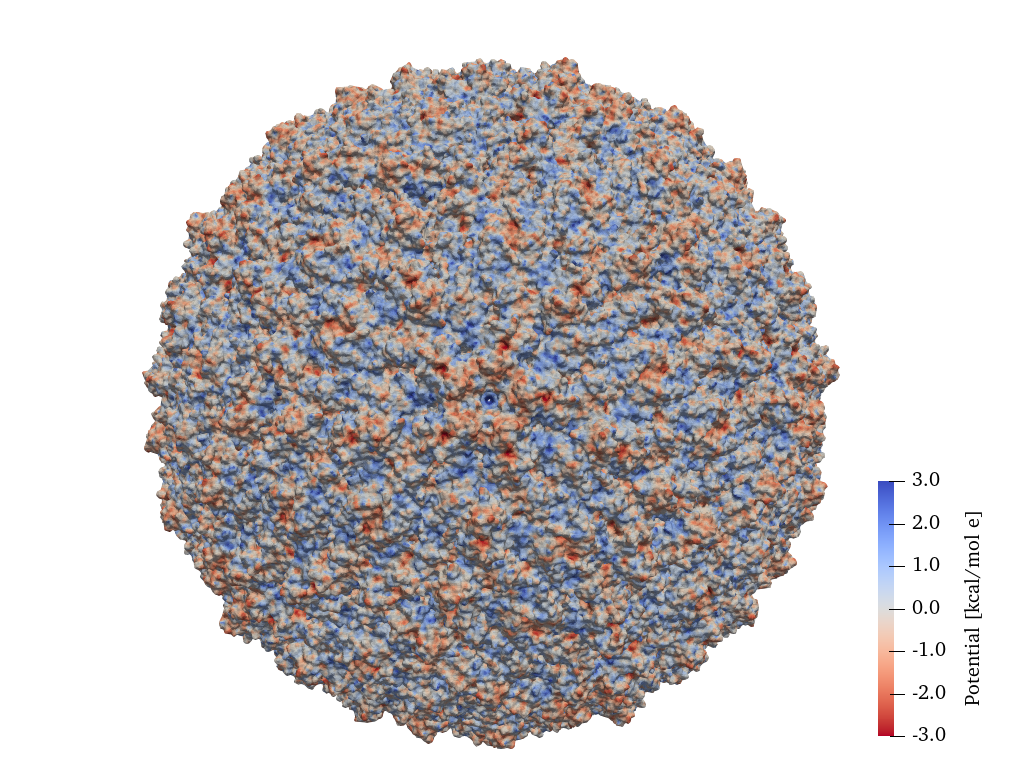
\includegraphics[width=0.75\textwidth]{6CO8_potential.png}
        \label{fig:6CO8_potential}}
    \caption{\textbf{a}, Structure of Zika virus (PDB code 6CO8) in assembly view. Each color indicates a polymer chain.
    \textbf{b}, Surface electrostatic potential of a Zika virus.
    The color bar is in units of [kcal/mol$\cdot$e].
    Visualization generated using ParaView.
    The starfish pattern seen in the polymer-chain colorization of Figure \ref{fig:6CO8_assembly} is faintly visible in the potential.
    }
\end{figure*}

Table \ref{tab:6CO8_result} summarizes the results and performance.
Again, we confirmed that the derivative formulation yields a well-conditioned system, which converged in 18 iterations and took less than 1.5 hours to solve.
By contrast, the direct formulation took almost twice as long to converge.

In this case, we also verified against \pygbe \cite{cooper2016pygbe}, a Python \bem library for biomolecular electrostatics.
Based on the solvation energy computed from \pygbe: $-117261.1$ [kcal/mol], the relative difference of our result is 0.6\% with the direct formulation and 0.9\% with the derivative formulation.
Figure \ref{fig:6CO8_potential} shows the computed electrostatic potential on the surface.

\paragraph{Reproducibility package}

Besides releasing all our software with an open-source license, we spared no effort to maximize the reproducibility of this work, compiling a ``repro-pack" in a version-control repository.
It contains all raw data from the experiments and a small Python package---\texttt{bempp\_pbs}, to facilitate running PB simulations with Bempp.
\texttt{bempp\_pbs} comprises a collection of scripts, including all post-processing scripts that are necessary to produce every result presented in this section, and driver and utility scripts for different formulations, with which readers can run these cases on their own hardware.
In addition, the ``repro-pack" also provides a Jupyter notebook for each study to generate secondary data and results.
The notebook corresponding to section \ref{result_conditioning} showcases how we could run a simple case of a spherical molecule using two formulations with just a few lines of code, and then compare their conditioning quantitatively with the help of other scientific Python tools.
These supplementary materials are included in our paper's GitHub repository at \href{https://github.com/barbagroup/bempp\_exafmm\_paper/}{https://github.com/barbagroup/bempp\_exafmm\_paper/}, which is also archived on Zenodo at \href{http://doi.org/10.5281/zenodo.4568951}{doi:10.5281/zenodo.4568951}.
We made separate archival deposits of input data (meshes and \texttt{pqr} files ) on the Zenodo service.
The deposit can be downloaded from \href{http://doi.org/10.5281/zenodo.4568768}{doi:10.5281/zenodo.4568768}.
